% vim:ft=tex
% rubber: module xelatex

\subsection{Stereo matching}
\label{sec:stereo}

\subsubsection{Implementation of dynamic programming}

We followed the methods described in \cite{realtimestereo} to implement dynamic programming for stereo matching.

In the simplest case, we do all of the following for each scanline of the image pair in turn.

Step 1: initialise disparity maps DisparityMapL and DisparityMapR.

Step 2: create a dynamic programming matrix A, whose dimensionality is equal to the scanline.

Initialise the top-left corner A[0,0] to zero. For all other elements of the matrix, evaluate them in order from upper left to lower right corner.

Step through the matrix and calculate
\[
A[i,j] = Minimum(A[i-1,j], A[i,j-1], A[i-1,j-1])  +  Difference(imageL, imageR)
\]
...where $Difference(imageL, imageR)$ is the difference between the i'th pixel of one image and the j'th pixel of the other.

Step 3: Once A has been filled, calculate a path of minimal cost through the matrix. In the simplest case, this is done by tracing back through the DP matrix starting at the bottom right corner A[n-1,n-1], and ending at A[0,0].

Choose the `path of least resistance', i.e. move up, left or up-left depending on $Minimum(A[i-1,j], A[i,j-1], A[i-1,j-1])$. Each time, fill in the disparity maps with your choice.

i.e.
DisparityMapL [i,y] = j-i
DisparityMapR [j,y] = i-j

Step 4: Once all this has been done for each scanline in the stereo pair, go through and map the lowest (possibly negative) disparity value to 0, and the highest disparity value to 255. This gives us our disparity map. Alternatively, the user can multiply by a fixed value.

...

That was the simplest case. In practise, we also have the options to:

(a) assign an additional bonus or penalty to moving diagonally in the dynamic programming matrix, depending on whether we want smooth or spiky (very disparate) images respectively,

(b) weight our choices for each scanline by those for the previous scanline, reducing error by `suggesting' ways to conform,

(c) run a median filter over the stereo images first to get rid of noise,

(d) not only run from bottom-right to top-left corner in the dynamic programming matrix, but also from top-left to bottom-right. We can choose the least-weight path overall. This helps reduce the cases where one of them goes horribly off the 'best' path because it followed the lowest-weight path into a dead end.

(e) improve running time by selecting a maximum disparity bound, b. The `path of least resistance' is never allowed to go outside this disparity bound because we set A[i,j] to a vast positive value if i > b or j > b.

%

One improvement we didn't implement: line skipping. (In that version, at thebeginning, every n’th horizontal line is calculated to find bounding space for possible disparities in between.)

%

\subsubsection{Testing of dynamic programming}

\begin{figure}[h]
  \centering
  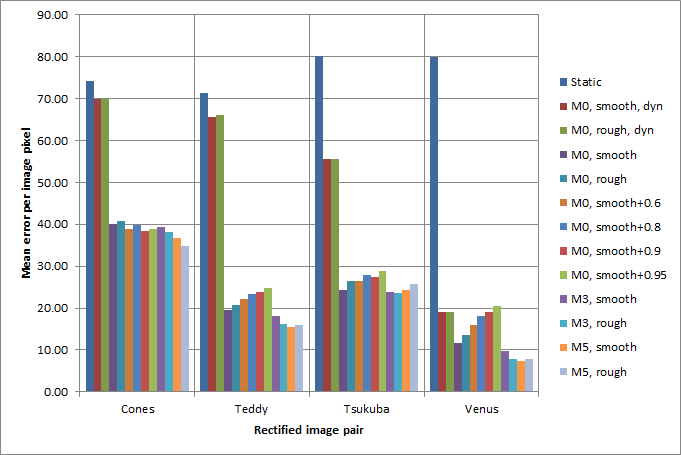
\includegraphics[width=0.8\textwidth]{Stereo-left-report}
  \caption[Results of dynamic programming (left image)]{Results of dynamic programming for the \emph{left} image, using various parameters. Resulting depth maps are compared to the canonical depth maps to obtain discrepancies (quantities of error). Each coloured column in the chart is a different parameterisation, as tested on one of the four images. `Static' is the baseline difference between the canonical depth map and a image with randomised values. `M0' indicates a median filter was not used in preprocessing. `M3' and `M5' indicate median filters of size 3 and 5 respectively. `rough' indicates scanlines did not influence each other. `smooth' indicates each scanline was influenced by the one previous, by 0.5 by default or by the amount given. `dyn' indicates the depth map was created by stretching the disparities to the full [0...255] range, instead of multiplying by the value recommended by \cite{middlebury} for each particular image.}
  \label{fig:stereo-left}
\end{figure}

\begin{figure}[h]
  \centering
  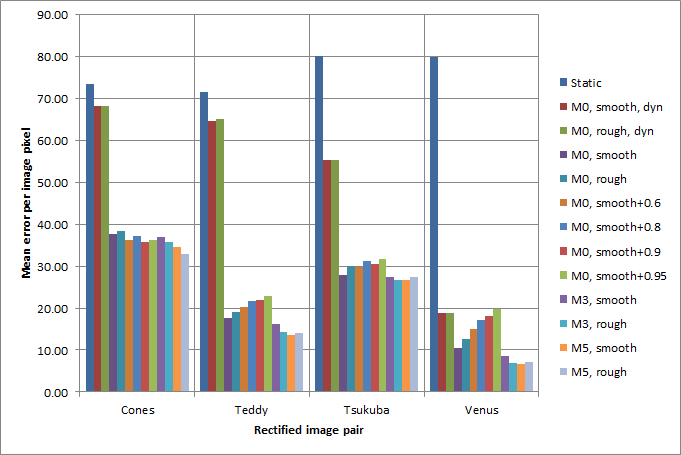
\includegraphics[width=0.8\textwidth]{Stereo-right-report}
  \caption[Results of dynamic programming (left image)]{Results of dynamic programming for the \emph{right} image, using various parameters. Resulting depth maps are compared to the canonical depth maps to obtain discrepancies (quantities of error). Each coloured column in the chart is a different parameterisation, as tested on one of the four images. `Static' is the baseline difference between the canonical depth map and a image with randomised values. `M0' indicates a median filter was not used in preprocessing. `M3' and `M5' indicate median filters of size 3 and 5 respectively. `rough' indicates scanlines did not influence each other. `smooth' indicates each scanline was influenced by the one previous, by 0.5 by default or by the amount given. `dyn' indicates the depth map was created by stretching the disparities to the full [0...255] range, instead of multiplying by the value recommended by \cite{middlebury} for each particular image.}
  \label{fig:stereo-right}
\end{figure}

See Figures~\ref{fig:stereo-left}~and~\ref{fig:stereo-right}.

We took the best results and submitted them to the Middlebury online tests. \cite{stereocorrespondence, middlebury} Their calculator unfortunately presupposes a cyclopean image, which we were not calculating. We submitted left and right instead, and chose the better of the two in each case. Still, we expect we would have scored considerably higher if we had calculated the cyclopean images. However, the details of our implementation made this difficult.

We had 44.9\% to 45.8\% bad pixels total. The worst Middlebury have on record is 20.7\%. \cite{stereocorrespondence, middlebury} For our test disparity maps, `Tsukuba' was best with 17.9\% error. `Venus' and `Teddy' were mediocre with 40.5\% and 54.4\% respectively. `Cones' was worst with 69.0\%.

\begin{figure}[h]
 \centering

 \subfloat[Tsukuba (rough)] { \label{fig:tsu-1} 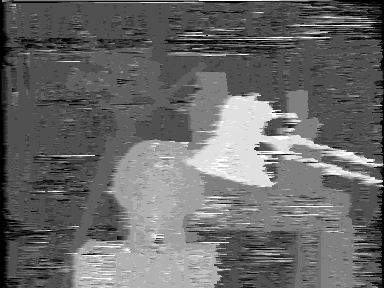
\includegraphics[trim = -2mm -2mm -2mm -2mm, width=0.23\textwidth]{stereo/tsu_imL_mat0_hardmult} }
 \subfloat[Venus (rough)] { \label{fig:ven-1} 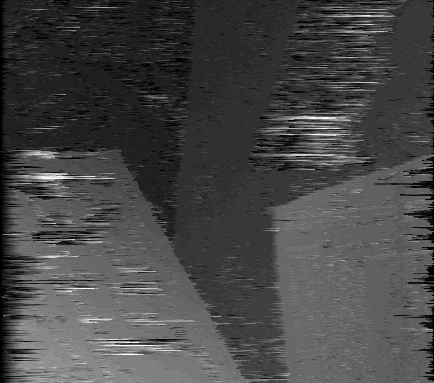
\includegraphics[trim = -2mm -2mm -2mm -2mm, width=0.23\textwidth]{stereo/ven_imL_mat0_hardmult} }
 \subfloat[Cones (rough)] { \label{fig:con-1} 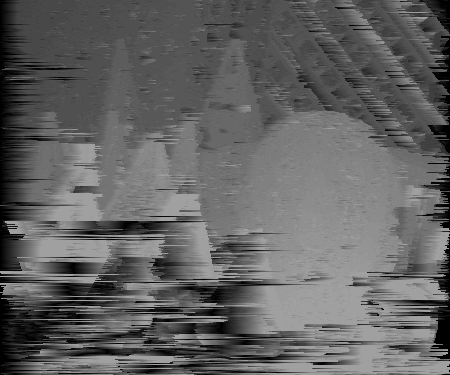
\includegraphics[trim = -2mm -2mm -2mm -2mm, width=0.23\textwidth]{stereo/con_imL_mat0_hardmult} }
 \subfloat[Teddy (rough)] { \label{fig:ted-1} 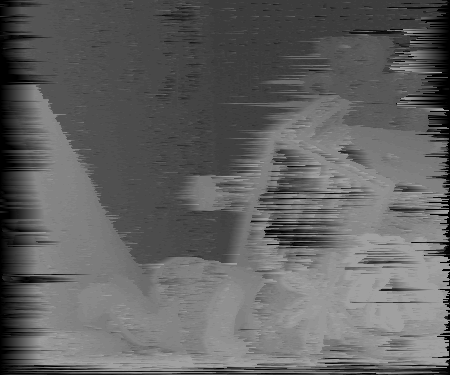
\includegraphics[trim = -2mm -2mm -2mm -2mm, width=0.23\textwidth]{stereo/ted_imL_mat0_hardmult} }\\

 \subfloat[Tsukuba (mid)] { \label{fig:tsu-2} 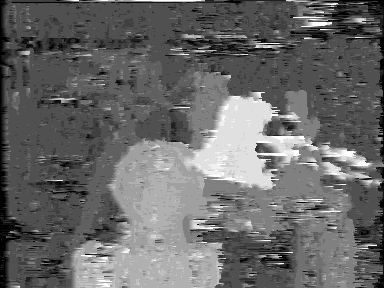
\includegraphics[trim = -2mm -2mm -2mm -2mm, width=0.23\textwidth]{stereo/tsu_imL_mat5_hardmult_smooth} }
 \subfloat[Venus (mid)] { \label{fig:ven-2} 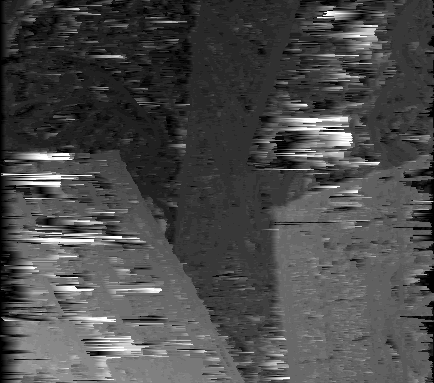
\includegraphics[trim = -2mm -2mm -2mm -2mm, width=0.23\textwidth]{stereo/ven_imL_mat5_hardmult_smooth} }
 \subfloat[Cones (mid)] { \label{fig:con-2} 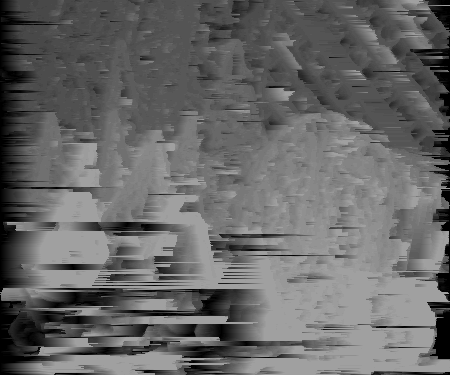
\includegraphics[trim = -2mm -2mm -2mm -2mm, width=0.23\textwidth]{stereo/con_imL_mat5_hardmult_smooth} }
 \subfloat[Teddy (mid)] { \label{fig:ted-2} 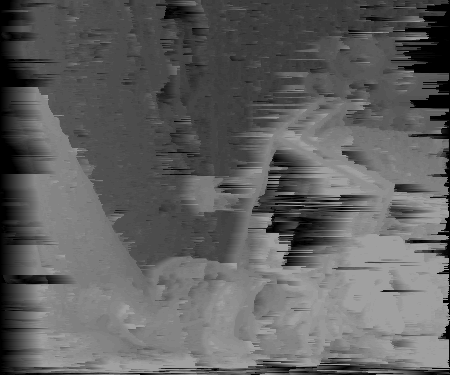
\includegraphics[trim = -2mm -2mm -2mm -2mm, width=0.23\textwidth]{stereo/ted_imL_mat5_hardmult_smooth} }\\

 \subfloat[Tsukuba (ideal)] { \label{fig:tsu-4} 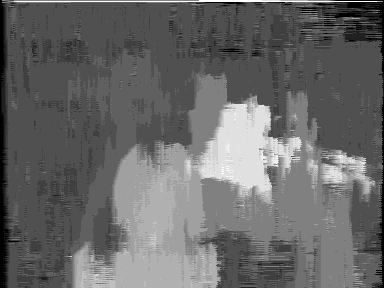
\includegraphics[trim = -2mm -2mm -2mm -2mm, width=0.23\textwidth]{stereo/tsu_imL_mat0_hardmult_smooth0.9} }
 \subfloat[Venus (ideal)] { \label{fig:ven-4} 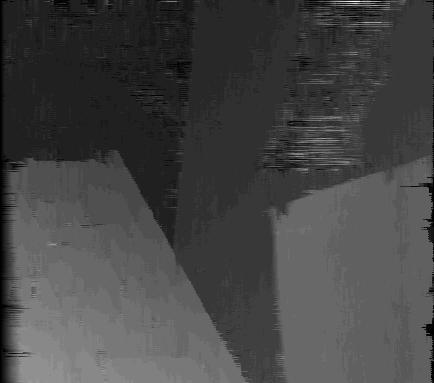
\includegraphics[trim = -2mm -2mm -2mm -2mm, width=0.23\textwidth]{stereo/ven_imL_mat0_hardmult_smooth0.9} }
 \subfloat[Cones (ideal)] { \label{fig:con-4} 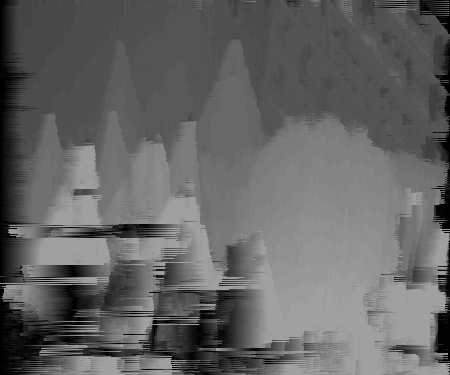
\includegraphics[trim = -2mm -2mm -2mm -2mm, width=0.23\textwidth]{stereo/con_imL_mat0_hardmult_smooth0.9} }
 \subfloat[Teddy (ideal)] { \label{fig:ted-4} 
\includegraphics[trim = -2mm -2mm -2mm -2mm, width=0.23\textwidth]{stereo/ted_imL_mat0_hardmult_smooth0.9} }

 \subfloat[Tsukuba (smooth)] { \label{fig:tsu-i} 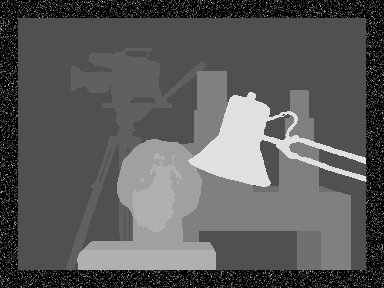
\includegraphics[trim = -2mm -2mm -2mm -2mm, width=0.23\textwidth]{stereo/tsu_ideal_L} }
 \subfloat[Venus (smooth)] { \label{fig:ven-i} 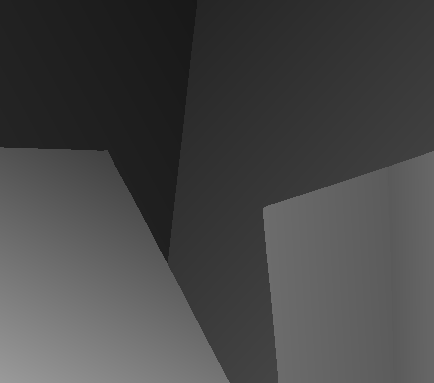
\includegraphics[trim = -2mm -2mm -2mm -2mm, width=0.23\textwidth]{stereo/ven_ideal_L} }
 \subfloat[Cones (smooth)] { \label{fig:con-i} 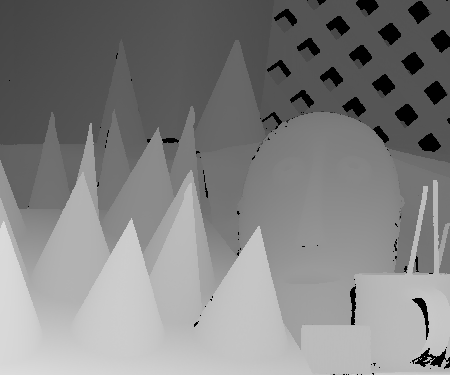
\includegraphics[trim = -2mm -2mm -2mm -2mm, width=0.23\textwidth]{stereo/con_ideal_L} }
 \subfloat[Teddy (smooth)] { \label{fig:ted-i} 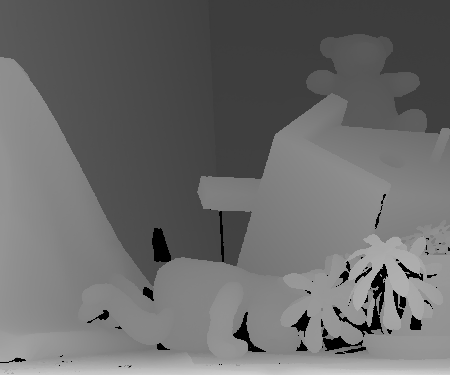
\includegraphics[trim = -2mm -2mm -2mm -2mm, width=0.23\textwidth]{stereo/ted_ideal_L} }\\

 \caption[Examples of dynamic programming with various parameters]{Examples of dynamic programming with various parameters. Canonical baseline images are courtesy of \citet{stereocorrespondence}.}
 \label{fig:stereo-image-depth-maps}
\end{figure}








